\chapter{Introduction}

In this chapter, we describe the classification problem that we will address in our term project (\autoref{sec:problemstatement}), we state the assumptions with which we will be working and give a brief overview of the strategy that we will follow, details of which can be found in (\autoref{sec:design}).

\begin{figure}[tbh!]
\centering
 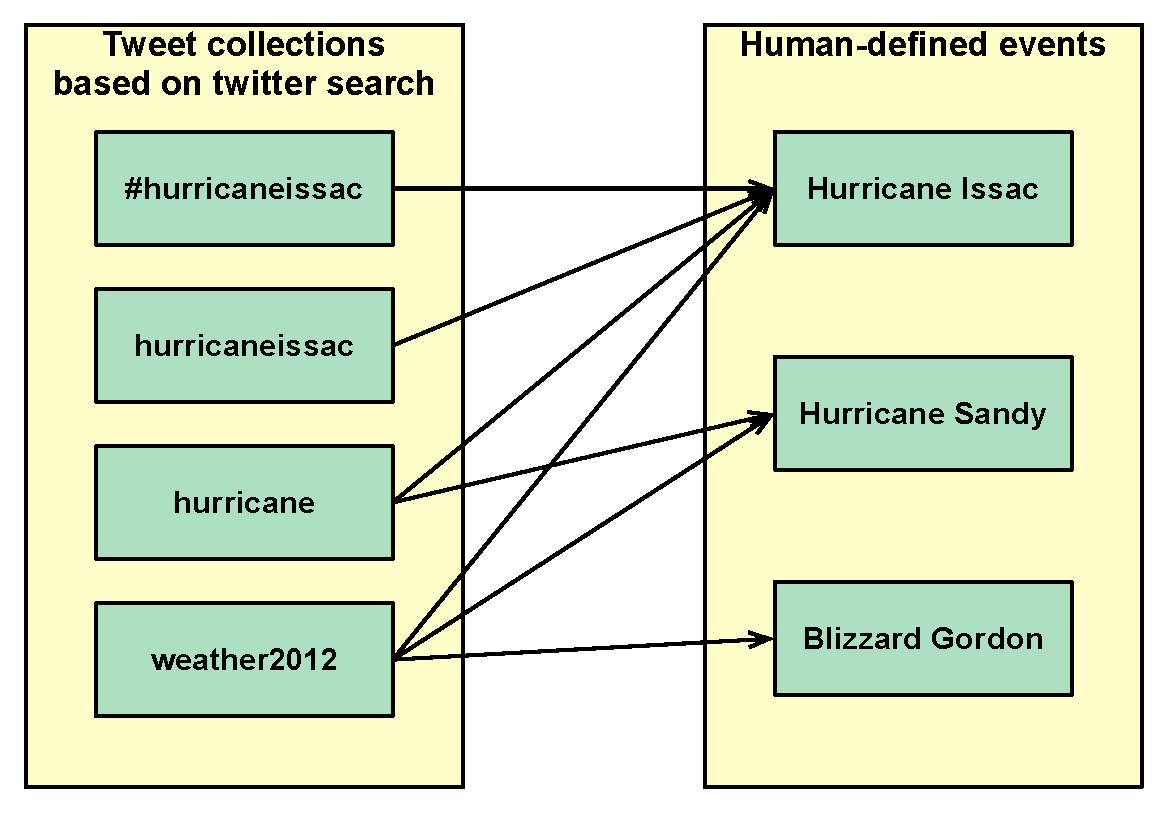
\includegraphics[width=0.5\textwidth]{figs/problem-statement.eps}
 \caption{\small Problem statement. \label{fig:statement}}
\end{figure}

\section{Requirements}
\label{sec:problemstatement}

The goal of the classification team is as follows:
 
\begin{quote}
Given a tweet collection and associated content from webpages linked in the tweets, and a set of events in the real world, we are to build a classifier that can classify the tweet and the webpages to a given event class.
\end{quote}
 
Figure~\ref{fig:statement} explains the problem  pictorially. Essentially, we have a collection of tweets  that have been retrieved based on keyword/tag search performed using the Twitter API. Additionally we have the content from webpages linked in the tweets. We will call this webpage and tweet collection together as documents in the remainder of this report, with exceptions to this convention noted explicitly. These are shown on the box on the left in Figure~\ref{fig:statement}. The human defined events or the real life events as stated in the goal are shown in the box on the right. The relationship between the collection of tweets and the events is many-to-many.

For instance, the tweet collection \fixed{weather2012} can have tweets related to the hurricanes ``Sandy'' and ``Issac'' as they occured in the same year and tweets from this collection can map to either ``Hurricane Sandy'' or ``Hurricane Issac'' event on the right. Likewise, for a given event, there can be several tweets that are associated with the event. We would also like to note that for a given event, just as there can be several tweets associated with the event, there can be multiple webpages that can be associated with the event. In a similar fashion, there could be websites that are comparing past with current events and could be classified in either event category.

For the task of classification, we make the following assumptions about the collection of tweets and webpages:
\begin{itemize}
\item Tweets have been extracted and are available as CSV files and some ``basic'' SPAM check has been done by tweet collection management team or by the teams from previous offerings of this course.
\item Webpage content will be extracted and be stripped of all tags and unrelated content by the website collection management team or by the teams from previous offerings of this course.
\item We will provide the Solr team with tweet id/webpage id and tags to classify the tweets and associated webpages.
\end{itemize}

More assumptions will be made as we make further progress on the project. We will now describe the approach that we will resort to from a very high level:

\begin{enumerate}
\item We start the process with a set of clean tweets and webpage content.
\item We perform some pre-processing to either load the data or extract only relevant parts of it.
\item Next we annotate the collection as either being relevant to a particular category or not.
\item We generate statistics related to the data obtained in step 2. 
\item The statistics are used to select features.
\item A training model is selected and using the annotated data and the set of features, its trained on.
\item This trained model is then used in classifying a larger collection of data.
\end{enumerate}

Additionally we may resort to other techniques such as bootstrap strategy to handle the larger datasets and these will become clearer in the weeks to come.
